\section{Evaluation}\label{sec:evaluation}

In this section, we compare the performance of state-of-the-art neural network accelerator designs and try to evaluate the techniques mentioned in section~\ref{sec:software} and section~\ref{sec:hardware}. \rev{We mainly reviewed the FPGA-based designs published in the top FPGA conferences (FPGA, FCCM, FPL, FPT), EDA conferences (DAC, ASPDAC, DATE, ICCAD), architecture conferences (MICRO, HPCA, ISCA, ASPLOS) since 2015. Because of the diversity in the adopted techniques, target FPGA chips, and experiments, we need a trade-off between the fairness of comparison and the number of designs we can use. In this paper, we pick the designs with 1) whole system implementation; 2) experiments on real NN models with reported speed, power, and energy efficiency.} 

The designs used for comparison are listed in Table~\ref{tab:hardware_list}. For data format, the "INT A/B" means that activations are A-bit fixed-point data and weights are B-bit fixed-point data. We also investigate the resource utilization and draw advice to both accelerator designers and FPGA manufacturers.

\begin{table}[htbp]
    \centering
    \caption{Performance and resource utilization of state-of-the-art neural network accelerator designs}
    \begin{tabular}{r|c|c|c|c|ccc|c}
        \toprule
        \multicolumn{1}{c|}{} & Data  & Speed & Power & Eff. & \multicolumn{3}{c|}{Resource(\%)} & \multirow{2}[4]{*}{FPGA chip} \\ %\cline{6-8}
        \multicolumn{1}{c|}{} & Format & (GOP/s) & (W)   & (GOP/J) & DSP   & logic & BRAM  &  \\
        \hline
            \cite{nakahara2017fully}    & 1bit      & 329.47    & 2.3   & 143.2 & 1     & 34    & 11    & Zynq XC7Z020 \\ 
            \cite{moss2017high}         & 1bit      & 40770     & 48    & 849.38 &   -   &   -   &   -   & GX1155 \\ 
            \cite{jiao2017accelerating} & 2bit      & 410.22    & 2.26  & 181.51 & 41   & 83    & 38    & Zynq XC7Z020 \\ 
            \cite{guo2017angel}         & INT8      & 84.3      & 3.5   & 24.1  & 87    & 84    & 89    & XC7Z020 \\ 
            \cite{suda2016throughput}   & INT16/8   & 117.8     & 19.1  & 6.2   & 13    & 22    & 65    & 5SGSD8 \\ 
            \cite{liu2016automatic}     & INT16/8   & 222.1     & 24.8  & 8.96  & 40    & 27    & 40    & XC7VX690T \\ 
            \cite{ma2017optimizing}     & INT16/8   & 645.25    & 21.2  & 30.43 & 100   & 38    & 70    & GX1150 \\             
            \cite{han2017ese}           & INT16/12  & 2520      & 41    & 61.5  & 54    & 89    & 88    & XCKU060 \\ 
            \cite{venieris2017fpgaconvnet} & INT16  & 12.73     & 1.75  & 7.27  & 95    & 67    & 6     & XC7Z020 \\ 
            \cite{qiu2016going}         & INT16     & 136.97    & 9.63  & 14.22 & 89    & 84    & 87    & XC7Z045 \\ 
            \cite{xiao2017exploring}    & INT16     & 229.5     & 9.4   & 24.42 & 92    & 71    & 83    & XC7Z045 \\ 
            \cite{zhang2016caffeine}    & INT16     & 354       & 26    & 13.6  & 78    & 81    & 42    & XC7VX690T \\ 
            \cite{guan2017fp}           & INT16     & 364.4     & 25    & 14.6  & 65    & 25    & 46    & 5SGSMD5 \\ 
            \cite{li2016high}           & INT16     & 565.94    & 30.2  & 22.15 & 60    & 63    & 65    & XC7VX690T \\ 
            \multirow{2}[2]{*}{\cite{Shen2018Towards}} & \multirow{2}[2]{*}{INT16} & 431  & 25 & 17.1  & 42 & 56 & 52    & XC7VX690T \\ %\cline{3-9}    
             &  & 785 & 26 & 30.2 & 53 & 8.3  & 30 & XCVU440 \\ %\hline
            \multirow{2}[2]{*}{\cite{zhang2016energy}} & \multirow{2}[0]{*}{INT16} & \multirow{2}[0]{*}{1280.3} & \multirow{2}[0]{*}{160} & \multirow{2}[0]{*}{8} & \multirow{2}[0]{*}{-} & \multirow{2}[0]{*}{-} & \multirow{2}[0]{*}{-} & XC7Z020+ \\
            &       &       &       &       &       &       &       & XC7VX690T$\times$6 \\ %\hline
            \cite{zhang2017improving}   & INT16     & 1790      & 37.46 & 47.8  & 91    & 43    & 53    & GX1150 \\ %\hline
            \cite{lu2017evaluating}     & INT16     & 2940.7    & 23.6  & 124.6 &   -   &   -   &   -   & ZCU102 \\ %\hline
            \cite{aydonat2017opencl}    & FP16      & 1382      & 45    & 30.7  & 97    & 58    & 92    & GX1150 \\ %\hline
            \cite{podili2017fast}       & INT32     & 229       & 8.04  & 28.5  & 100   & 84    & 18    & Stratix V \\ %\hline            
            \cite{guan2017fpga}         & FP32      & 7.26      & 19.63 & 0.37  & 42    & 65    & 52    & XC7VX485T \\ %\hline
            \cite{zhang2015optimizing}  & FP32      & 61.62     & 18.61 & 3.3   & 80    & 61    & 50    & XC7VX485T \\ %\hline
            \cite{zhang2017frequency}   & FP32      & 123.5     & 13.18 & 9.37  & 88    & 85    & 64    & Stratix V \\ %\hline
            \cite{zhang2017improving}   & FP32      & 866       & 41.73 & 20.75 & 87    & -     & 46    & GX1150 \\ 
            \bottomrule
        \end{tabular}%
    \label{tab:hardware_list}%
  \end{table}%

\begin{figure}[ht]
    \centering
    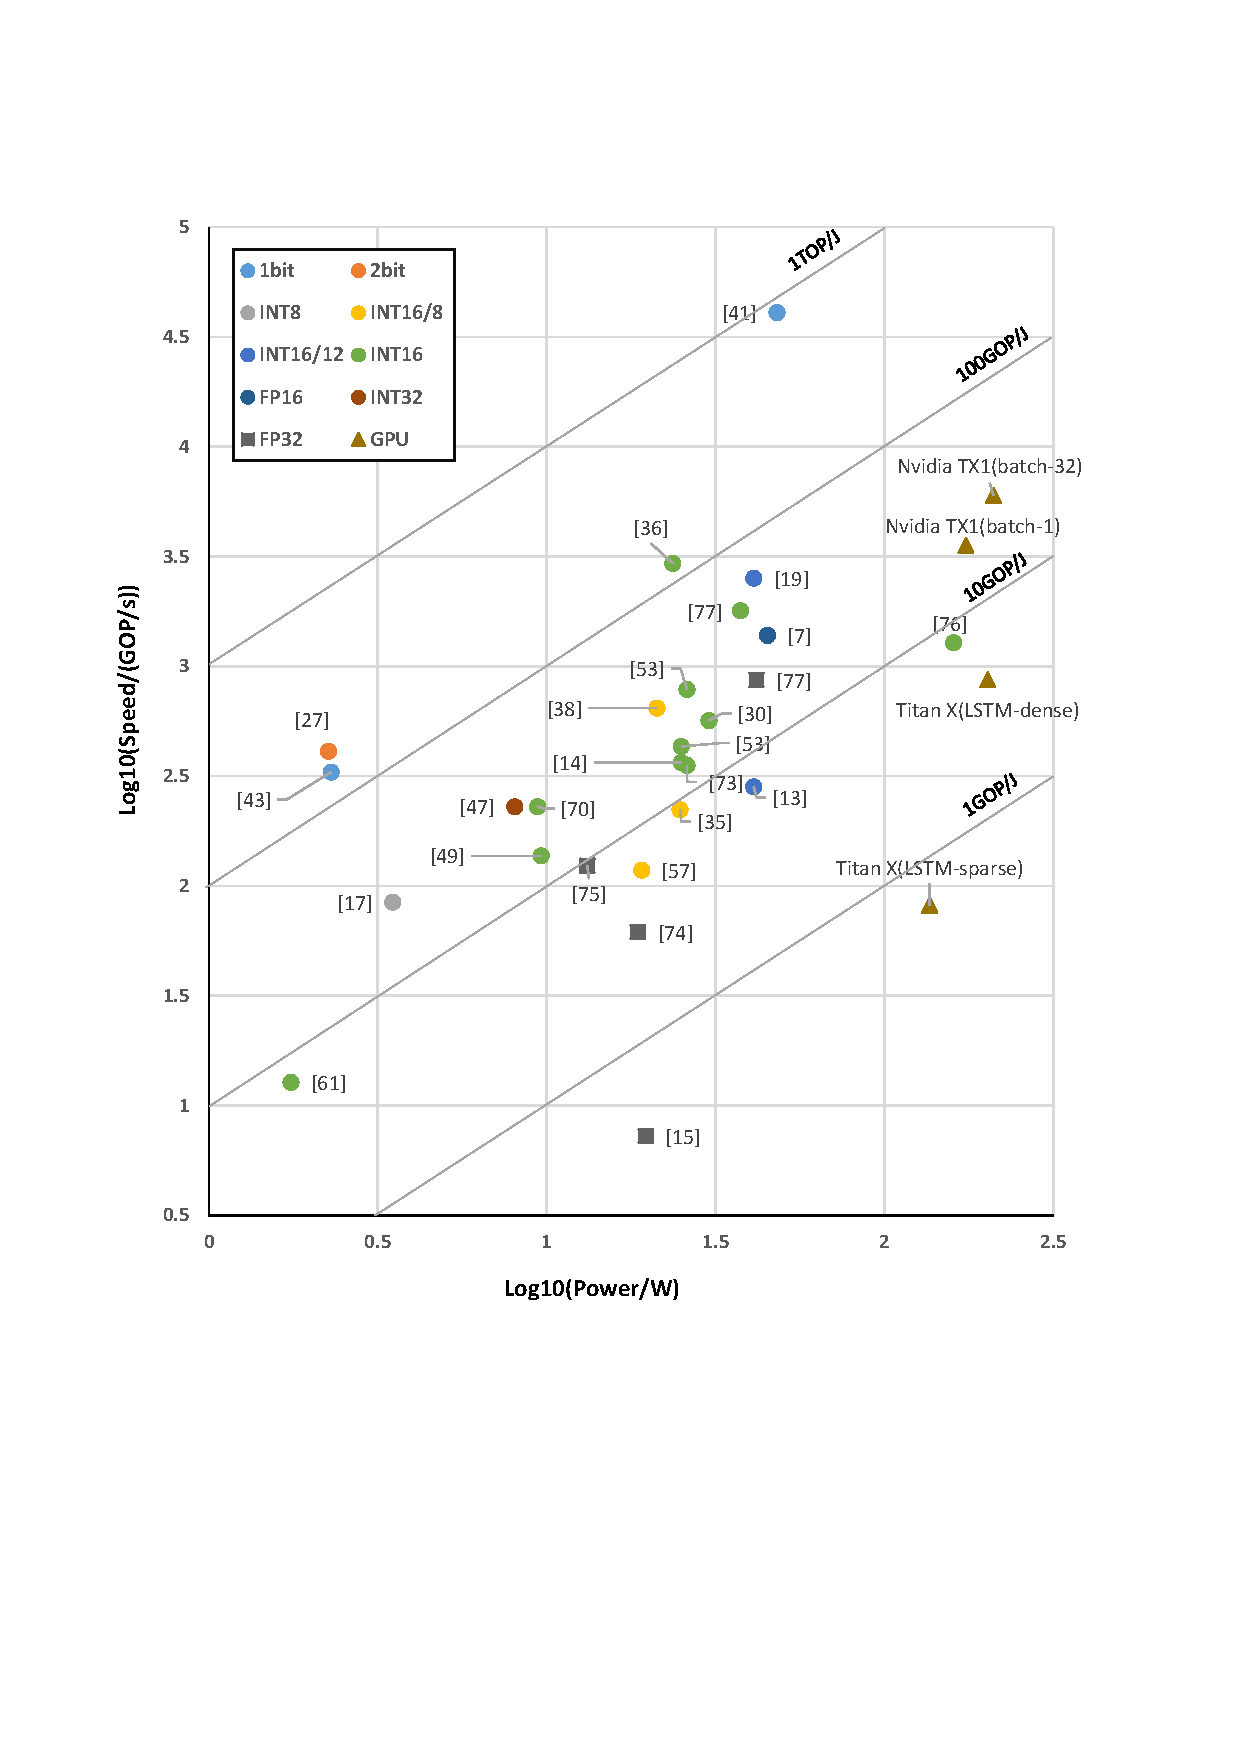
\includegraphics[width=1.0\columnwidth]{fig/efficiency.pdf}
    \caption{A comparison between different designs on a logarithm coordinate of power and performance. }
    \label{fig:efficiency}
\end{figure}

\begin{figure}[ht]
    \centering
    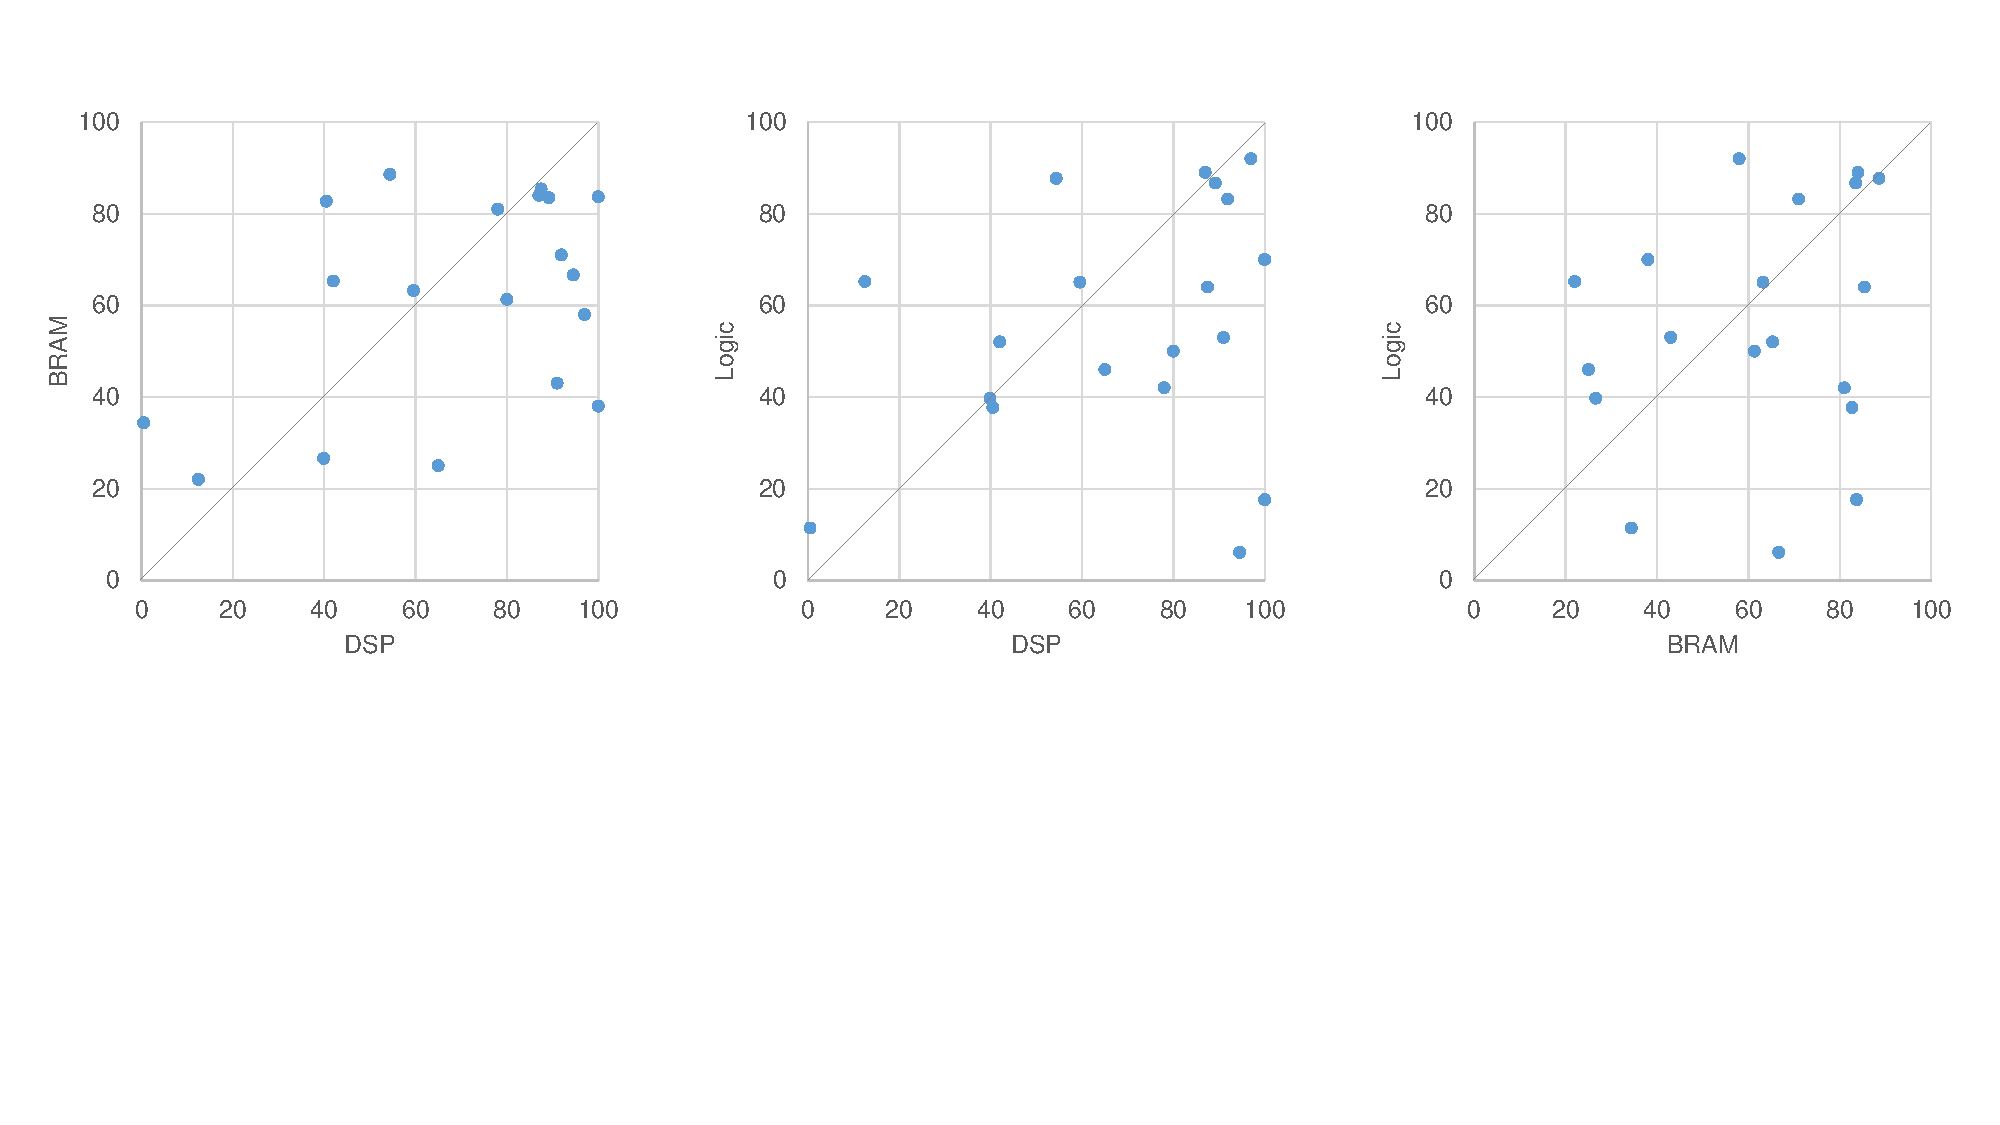
\includegraphics[width=1.0\columnwidth]{fig/resource.pdf}
    \caption{Resource utilization ratio of different accelerator designs.}
    \label{fig:resource}
\end{figure}

Each of the designs in Table~\ref{tab:hardware_list} drawn as a point in Figure~\ref{fig:efficiency}, using $log_{10}(power)$ as $x$ coordinate and $log_{10}(speed)$ as $y$-axis. Therefore, $y-x=log_{10}(energy\_efficiency)$. Besides the FPGA based designs, we also plot the GPU experimental results used in \cite{guo2017angel, han2017ese} as standards to measure the FPGA designs' performance.

\rev{\subsubsection*{\textbf{Bit-width Reduction}} Among all the designs, 1-2 bit based designs~\cite{jiao2017accelerating, moss2017high, nakahara2017fully} show outstanding speed and energy efficiency. This shows that extremely low bit-width is a promising solution for high-performance design. As introduced in section~\ref{sec:software:quant}, linear quantized 1-2 bit network models suffer from great accuracy loss. Further developing related accelerator will be of little use. More efforts should be put on the models. Even trading speed with accuracy can be acceptable considering the current hardware performance.

Besides the 1/2bit designs, the rest of the designs adopts 32-bit floating-point data or linear quantization with 8 or more bits. According to the results in section~\ref{sec:software:quant}, within 1\% accuracy loss can be achieved. So we think the comparison between these designs is fair in accuracy. INT16/8 and INT16 are commonly adopted. But the difference between these designs is not obvious. This is because the underutilization of DSPs discussed in section~\ref{sec:hardware:cu:lbu}. The advantage of INT16 over FP32 is obvious except for \cite{zhang2017improving}, where the hard-core floating-point DSPs are utilized. To a certain extent, this shows the importance of fully utilizing the DSPs on-chip.}

\subsubsection*{\textbf{Fast Convolution Algorithm}} Among all the 16-bit designs, \cite{lu2017evaluating} achieves the best energy efficiency and the highest speed with the help of the $6\times 6$ Winograd fast convolution, which is $1.7\times$ faster and $2.6\times$ energy efficient than the 16-bit design in \cite{zhang2017improving}. The design in \cite{zhang2017frequency} achieves $2\times$ speedup and $3\times$ energy efficiency compared with \cite{zhang2015optimizing} where both designs use 32-bit floating-point data. Overall, the improvement does not match the estimation but can still reach 2-3$\times$.

\subsubsection*{\textbf{System Level Optimization}} The overall system optimization is not well addressed in most of the work. As this is also related to the HDL design quality, we can roughly evaluate the effect. Here we compare three designs\cite{zhang2016caffeine, liu2016automatic, li2016high} on the same XC7VX690T platform and try to evaluate the effect. All the three designs implement 16-bit fixed-point data format except that ~\cite{liu2016automatic} uses 8-bit for weights. No fast convolution or sparsity is utilized in any of the work. Even though, \cite{li2016high} achieves $2.5\times$ the energy efficiency of \cite{liu2016automatic}. It shows that a system level optimization has a strong effect even comparable to the use of fast convolution algorithm. 

We also investigate the resource utilization of the designs in Table~\ref{tab:hardware_list}. Three kinds of resources (DSP, BRAM, and logic) are considered. We plot the designs in Figure~\ref{fig:resource} using two of the utilization ratio as x and y coordinate. We draw the diagonal line of each figure to show the designs' preference on hardware resource. The BRAM-DSP figure shows an obvious preference on DSP over BRAM. A similar preference appears on DSP over logic. This indicates that current FPGA designs are more likely computation bounded. FPGA manufacturers targeting neural network applications can adjust the resource allocation accordingly.

\subsubsection*{\textbf{Comparision with GPU}} In general, FPGA based designs have achieved comparable energy efficiency to GPU with 10-100GOP/J. But the speed of GPUs still surpasses FPGAs. Scaling up the FPGA based design is still a problem. Zhang et al.~\cite{zhang2016energy} propose the FPGA-cluster-based solution using 16-bit fixed-point computation. But the energy efficiency is worse than the other 16-bit fixed-point designs. 

\rev{Here we estimate the achievable speed of an ideal design. We use the 16-bit fixed-point design in~\cite{lu2017evaluating} as a baseline, which is the best 16-bit fixed-point design with both the highest speed and energy efficiency. 8-bit linear quantization can be adopted according to the analysis in section~\ref{sec:software:quant}, which achieves another $2\times$ speedup by utilizing 1 DSP as 2 multipliers. Fast convolution and frequency optimization further improve the system by $4\times$ and $2\times$ respectively. Consider a sparse model which is similar to the one in~\cite{han2017ese} with 10\% non-zero values. We can estimate a similar $6\times$ improvement as~\cite{han2017ese}. In general about $12\times$ speedup and better energy efficiency can be achieved, which means 36TOP/s speed with about 50W. This shows that it is possible to achieve over $10\times$ higher energy efficiency on FPGA over 32-bit floating-point process on GPU.

The left problem is: does all the techniques: reuse of DSP, sparsification, quantization, fast convolution work well together? Pruning a single element in a 2D convolution kernel is of no use for fast convolution because the 2D kernel is always processed as a whole. Directly pruning 2D kernels as a whole may help. But the reported accuracy of this method is lower~\cite{Mao2017Exploring} than a fine-grained pruning. The irregular data access pattern for processing sparse network and the increase in parallelism also brings challenges to the design of memory system and scheduling strategy.}

